\documentclass{article}
\usepackage{iclr2027_conference,times}
\usepackage[T1]{fontenc}
\usepackage{amsmath,amssymb,booktabs,tabularx,microtype}
\usepackage{graphicx}
\usepackage{float}
\usepackage{hyperref}
\usepackage{url}
\hypersetup{hidelinks}
\usepackage[section]{placeins}
\usepackage{tikz}
\usetikzlibrary{arrows.meta,positioning}
\setlength{\emergencystretch}{2em}
\title{SCD: Spatial Concept Distillation\\for Spurious-Correlation Robustness\\in Self-Supervised Pretraining}
\author{}
\begin{document}
\maketitle
\begin{abstract}
Self-supervised representations inherit the co-occurrences of their unlabeled training images: when cats appear mostly indoors, an encoder trained from scratch learns indoor scenes as evidence for cats. We introduce Spatial Concept Distillation (SCD), which uses sparse, language-aligned concepts to tell the encoder \emph{where} each concept sits in an image. A frozen CLIP/SpLiCE teacher names the concepts of the training set, groups synonyms into concept factors and computes a dense map of every factor for every training image. During SimCLR pretraining, each location of the student's last feature map has to predict the concept values at its place in the view, through a ridge regression cross-fitted between two halves of the batch, so memorizing individual images lowers no part of the loss. Every concept is treated alike: no step decides which concept is the class and which the spurious attribute and no target or group annotation enters pretraining. Only the student encoder is needed at inference. On Waterbirds and MetaShift (six seeds) and Spur-CIFAR10 (two seeds), SCD raises validation worst-group accuracy over SimCLR by 6.1, 6.8 and 22.5 points, while the same loss with another image's maps stays at the SimCLR level. Dense CLIP components in place of named concepts match SCD on Waterbirds and fall to the SimCLR level on MetaShift. The student's concept scores still follow the training co-occurrence, so SCD strengthens the core feature without separating it from its usual context.
\end{abstract}

\section{Introduction}
An image can contain several predictive factors. In Waterbirds, bird category correlates with background in the training set; in MetaShift, 88\% of the training cats sit indoors and 88\% of the dogs outdoors. A representation that strongly encodes this association can fail on birds shown in an uncommon environment or on cats on a lawn. Worst-group evaluation makes these failures visible even when aggregate accuracy appears acceptable \citep{sagawa2020groupdro}. Self-supervised pretraining inherits the correlations present in its unlabeled images and standard view augmentation leaves open which context changes should preserve object identity.

Our goal is to learn a visual encoder whose downstream predictions remain useful when object--context associations change, using no target labels or group annotations during pretraining and no knowledge of which concept is spurious. Deep feature reweighting shows that a linear head retrained on a small group-balanced set recovers worst-group accuracy whenever the representation encodes the core feature apart from the spurious one \citep{kirichenko2023dfr}. A frozen vision-language model supplies semantic structure learned from external data and SpLiCE exposes this structure as sparse non-negative coordinates associated with text concepts \citep{bhalla2024splice}. We hypothesize that the location of a concept is the missing signal: at the image level cat and couch appear together, while at the pixel level they occupy different places in every image.

SCD turns the concepts of the training set into dense maps with a frozen CLIP model and asks every location of the student's last feature map to predict the concept values at its place in the view. A ridge regression fitted on one half of the batch scores the other half, so only concept directions shared across images lower the loss. During inference only the trained encoder and downstream classifier are required.

Our contribution is a prior-free spatial concept loss for self-supervised pretraining and a controlled study of its effect on worst-group accuracy. The study separates the concept content of the maps (shuffled maps), the role of named concepts against generic dense CLIP information (principal-component maps) and the role of location (image-level concept regression). A post-hoc audit measures which concepts the student carries to unseen images and whether it separates them from their usual context.

\section{Related Work}
\paragraph{Dense and region-level self-supervised learning.}
SimCLR contrasts two views of an image against the other images in the batch \citep{chen2020simclr} and pools the feature map before its projection head. DenseCL adds a contrastive loss between matched locations of the two views \citep{wang2021densecl} and PixPro asks locations that cover the same image pixels to agree \citep{xie2021pixpro}. DetCon pools the feature map inside unsupervised masks and contrasts the pooled regions across views \citep{henaff2021detcon}. These methods supervise locations with the student's own features or with unnamed segments. SCD supervises every location with named concept values from a frozen teacher and keeps the SimCLR objective unchanged.

\paragraph{Dense concepts from vision-language models.}
CLIP supplies a shared image--text space \citep{radford2021clip}. MaskCLIP shows that its patch tokens align with text embeddings once the last attention pooling is bypassed \citep{zhou2022maskclip} and ClearCLIP obtains cleaner maps by removing the residual and feed-forward branches of the last block and using query--query attention \citep{lan2024clearclip}. SCD uses the ClearCLIP construction offline, on the training images only. Feature distillation from CLIP into a smaller student works with plain feature mimicry \citep{yang2024clipkd} and AM-RADIO distils several teachers with summary and spatial losses \citep{ranzinger2024radio}. SCD distils a low-dimensional concept map through a regression that is refitted in every batch, in the manner of differentiable closed-form solvers in meta-learning \citep{bertinetto2019r2d2,lee2019metaoptnet}.

\paragraph{Concept representations, discovery and editing.}
TCAV measures prediction sensitivity along directions learned from concept examples \citep{kim2018tcav}; ACE discovers visual concepts by clustering image segments in feature space \citep{ghorbani2019ace}. Concept Bottleneck Models route predictions through annotated attributes that can be edited \citep{koh2020cbm}. Post-hoc Concept Bottleneck Models add an editable concept layer to pretrained representations \citep{yuksekgonul2023pcb}; Label-Free Concept Bottleneck Models use language-derived concepts without manual concept annotations \citep{oikarinen2023lfcbm}. These methods clarify different roles for concepts: explanation, prediction and intervention. SpLiCE expresses CLIP embeddings as sparse non-negative combinations of named text directions \citep{bhalla2024splice}. SCD uses these coordinates to choose the vocabulary of concepts whose locations the student learns.

\paragraph{Spurious features and invariance in SSL.}
Contrastive learning can suppress harder features in favour of shortcut solutions. Implicit feature modification counteracts this through feature-space perturbations of the contrastive comparison \citep{robinson2021shortcut}. Content--style identifiability results explain how augmentation can isolate invariant content under explicit assumptions about the data-generating process \citep{vonkugelgen2021content} and correlations between generative factors in the training data persist in the learned latents \citep{trauble2021correlated}. Learning-speed-aware SSL (LA-SSL) emphasizes slowly learned examples through adaptive sampling \citep{zhu2023lassl}. LateTVG prunes late layers of the encoder to form a second view that discards the easiest features \citep{hamidieh2024latetvg}. Background augmentations swap or remove salient backgrounds during SSL \citep{ryali2021background}. LA-SSL and LateTVG assume that the spurious feature is the easy one and background augmentation assumes that it is the background. SCD makes no assumption about which concept is spurious.

\paragraph{Robustness with other supervision regimes.}
Group DRO uses annotated groups \citep{sagawa2020groupdro}, while Just Train Twice upweights errors of an initial supervised classifier \citep{liu2021jtt}. GALS grounds a language description of the class in CLIP attention and guides a supervised network towards those pixels \citep{petryk2022gals}, a descendant of explanation constraints from annotated masks \citep{ross2017rrr}. CoBalT discovers concepts without labels and uses them to balance supervised training \citep{arefin2024cobalt}. DIAL uses sparse-autoencoder analysis to remove spurious directions from VLM representations \citep{yalavarthi2026dial}. SCD shares the use of language-grounded locations with GALS, but it names no class and trains a separate encoder without labels. Supervised group-robust and zero-shot VLM accuracies of the above papers therefore offer no matched numerical comparisons to our training pipeline.

\section{Problem Setting}
Let $\mathcal{D}=\{x_i\}_{i=1}^{N}$ be unlabeled training images with stable sample identifiers. The learned representation is $f_\theta(x)$. A downstream classifier $w$ predicts target $y$ from frozen features. For evaluation groups $g=(y,a)$ defined by target and spurious attribute $a$, we report empirical average accuracy and worst-group accuracy:

\begin{equation}
 \mathrm{Avg}=\frac{1}{n}\sum_{i=1}^{n}\mathbf{1}\{w(f_\theta(x_i))=y_i\},\qquad
 \mathrm{WGA}=\min_g\frac{1}{n_g}\sum_{i:g_i=g}\mathbf{1}\{w(f_\theta(x_i))=y_i\}.
\end{equation}

Concept discovery, map construction and SSL use images and frozen representations. Labels and group annotations enter downstream probe fitting, balanced probe-subset construction and post-hoc analysis. ``Label-free'' in our work refers to the concept and SSL stages; CLIP's external image--text pretraining and the supervised evaluation stage use labels. We add one restriction: the method may use no knowledge of which concept is the target and which the spurious attribute, since that knowledge differs between datasets (the background in Waterbirds, gender in CelebA with hair colour as the target). Every concept therefore enters the loss in the same way.

\section{Method}
SCD has four stages: encode images as sparse named concepts; group the concepts into factors that name one thing each; map every factor densely over every training image; and train a SimCLR student whose feature map predicts the warped maps of its views. The frozen branch runs once on the training images. It provides the student with the location of every concept, without any target or spurious information (Figure~\ref{fig:architecture}).

\begin{figure}[htbp]
\centering
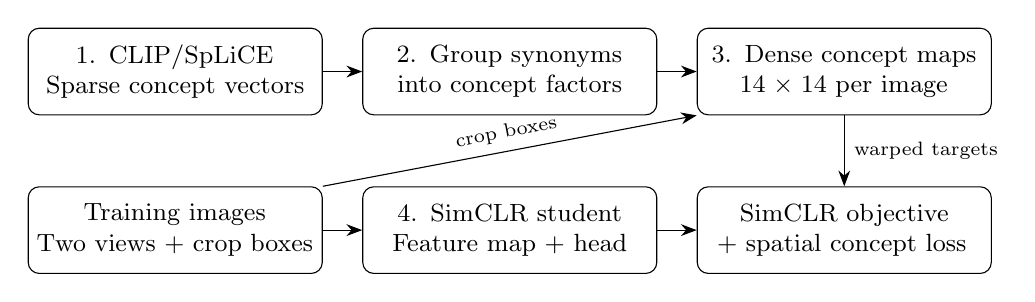
\begin{tikzpicture}[node distance=5mm and 5mm,
 box/.style={draw,rounded corners,align=center,font=\small,minimum height=11mm,text width=35mm},
 >={Stealth[length=2mm]}]
\node[box] (teacher) {1. CLIP/SpLiCE\\Sparse concept vectors};
\node[box,right=of teacher] (groups) {2. Group synonyms\\into concept factors};
\node[box,right=of groups] (maps) {3. Dense concept maps\\$14\times14$ per image};
\node[box,below=9mm of teacher] (views) {Training images\\Two views + crop boxes};
\node[box,right=of views] (student) {4. SimCLR student\\Feature map + head};
\node[box,right=of student] (loss) {SimCLR objective\\+ spatial concept loss};
\draw[->] (teacher)--(groups); \draw[->] (groups)--(maps);
\draw[->] (views)--(student); \draw[->] (student)--(loss);
\draw[->] (maps)--node[right,font=\scriptsize]{warped targets}(loss);
\draw[->] (views.north east)--node[above,sloped,font=\scriptsize]{crop boxes}(maps.south west);
\end{tikzpicture}
\caption{The four-stage pipeline. Training images enter both the frozen teacher branch and the student branch. Concept discovery, map construction and SSL use no target or group annotations and no concept type. At inference the teacher, the maps and the SSL heads are discarded; a supervised linear probe evaluates the frozen student backbone.}
\label{fig:architecture}
\end{figure}

\subsection{Stage 1: SpLiCE concept representation}
SpLiCE provides a sparse vector whose non-negative coordinates measure contributions of CLIP text directions to an image embedding. These coordinates give a vocabulary of the concepts that actually occur in the training set, without first annotating which concepts are spurious.

Given an image $x_i$, frozen CLIP produces an embedding $z_i$. We center and normalize it using the fixed SpLiCE mean $\mu$. With a row-normalized text dictionary $D\in\mathbb{R}^{K\times d}$, positive sparse regression gives
\begin{equation}
 u_i=\operatorname{norm}(z_i-\mu),\qquad
 c_i\in\arg\min_{c\geq0}\|u_i-D^\top c\|_2^2+\lambda_1\|c\|_1.
\end{equation}
All vectors are columns and \(\operatorname{norm}(v)=v/\lVert v\rVert_2\). Obtained concept decomposition $c_i$ of image $x_i$ can be read directly as a set of active concept coordinates. For example, if the dictionary contains the concepts \emph{lawn}, \emph{cat} and \emph{alien}, one image might yield
\[
c_i =
0.72\,e_{\text{lawn}}
+ 0.41\,e_{\text{cat}}
+ 0.18\,e_{\text{alien}},
\]
with most remaining coordinates equal to zero, where $e_k$ denotes the
coordinate associated with concept $k$.

\subsection{Stage 2: Concept factors}
Words from dictionary $D$ often name one visual content several times (\emph{cat}, \emph{kitten}, \emph{kitty}). The L1 penalty of SpLiCE activates one of two synonyms per image, so synonyms rarely co-activate and their centred dictionary directions can lie far apart. We therefore group concepts by their raw CLIP text embeddings $t_k$, which keep synonyms close (cosine 0.85 to 0.94) and separate an object from its usual context (0.64 to 0.72). We keep concepts active on 0.2\% to 95\% of the training images and define the similarity of two concepts as
\begin{equation}
 s_{k\ell}=
 \begin{cases}
 \cos(t_k,t_\ell) & \text{if } \rho_{k\ell}\geq\tau_\rho,\\
 -1 & \text{otherwise,}
 \end{cases}
\end{equation}
where $\rho_{k\ell}$ is the correlation across training images of their responses $u_i^\top d_k$ and $u_i^\top d_\ell$. Average-linkage clustering on $1-s_{k\ell}$, cut at distance $1-\tau_t$, forms the concept groups. Average linkage joins two clusters only when their members agree on average, which stops the chains that a union of pairwise matches forms through a bird and its background.

A concept factor $F$ is one group. Its activation on image $x_i$ is $a_{iF}=\sum_{k\in F}c_{ik}$ and we keep the factors active on 2\% to 90\% of the training images. Its text direction is the normalized mean of its members' raw text embeddings, $d_F=\operatorname{norm}\big(\tfrac{1}{|F|}\sum_{k\in F}\operatorname{norm}(t_k)\big)$. Waterbirds has 242 factors, MetaShift 130 and Spur-CIFAR10 147. Exact thresholds are given in Appendix~\ref{app:provenance}.

\subsection{Stage 3: Dense concept maps}
For every training image we compute where each factor sits. Following ClearCLIP \citep{lan2024clearclip}, the last transformer block of CLIP replaces its query--key attention by query--query attention and drops its residual and feed-forward branches. With $X$ the normalized tokens entering this block, the patch embeddings in the text space are
\begin{equation}
 P=\operatorname{norm}\!\Big(\operatorname{LN}\big(\operatorname{softmax}(QQ^\top/\sqrt{d_h})\,V\,W_O\big)\,W_{\mathrm{proj}}\Big),
 \qquad Q=XW_Q,\; V=XW_V,
\end{equation}
applied per attention head and normalized per patch. Images are read at 448 pixels through 224-pixel windows with a stride of 112 pixels; window scores are averaged where windows overlap and pooled to a $14\times14$ grid. At every cell $u$ the map is a softmax over the factors,
\begin{equation}
 M_{iF}(u)=\frac{\exp\!\big(\cos(p_i(u),d_F)/T\big)}{\sum_{G}\exp\!\big(\cos(p_i(u),d_G)/T\big)},
\end{equation}
with temperature $T=0.01$, so each cell distributes one unit of mass over the factors (Figure~\ref{fig:examples}). Each factor's map is then standardized over all images and cells, $\tilde M_{iF}=(M_{iF}-m_F)/s_F$. The maps take 40 seconds to compute for MetaShift on one GPU and are stored once.

\subsection{Stage 4: Cross-fitted spatial concept loss}
The standard two-view SimCLR objective remains unchanged. The SSL transform records the crop box and flip of every view $x_i^{(v)}$ and RoIAlign cuts the view's part out of $\tilde M_i$ and resizes it to the student's last feature map, giving targets $Y_i^{(v)}\in\mathbb{R}^{K\times h\times w}$. The feature map $H_i^{(v)}\in\mathbb{R}^{C\times h\times w}$ is the output of the last ResNet stage before global pooling ($7\times7\times512$ for 224-pixel views).

Every location $u$ gives a unit-norm feature row $r=\operatorname{norm}(H_i^{(v)}(u))$ and a target $y=Y_i^{(v)}(u)$. A trained linear head on these rows could store a target per image: on the 1,700 MetaShift images, image-level heads fit shuffled targets almost as well as real ones. We therefore split the images of a batch into halves $A$ and $B$, with both views of an image in one half and fit a ridge regression on the locations of $A$ in closed form,
\begin{equation}
 W_A=\big(\bar R_A^\top\Omega_A\bar R_A+\rho I\big)^{-1}\bar R_A^\top\Omega_A\big(Y_A-\bar y_A\big),
\end{equation}
where $\bar R_A$ stacks the rows of $A$ centred by their weighted mean $\bar r_A$, $\Omega_A$ holds the per-view loss weights and $\rho$ is an absolute ridge. The fit predicts every location of $B$, $\hat Y_B=(R_B-\bar r_A)W_A+\bar y_A$ and the reverse fit predicts $A$. The loss is the held-out squared error,
\begin{equation}
 \mathcal{L}_{\mathrm{spatial}}=\frac{1}{2}\sum_{(S,S')\in\{(A,B),(B,A)\}}
 \frac{\sum_{v\in S'}\omega_v\,\frac{1}{hwK}\big\lVert\hat Y_v-Y_v\big\rVert_2^2}{\sum_{v\in S'}\omega_v}.
\end{equation}
Gradients pass through the solve and the prediction. A feature that identifies one image carries nothing to the other half; only concept directions shared across images lower the loss.

A fixed fifth of the training images carries loss weight $\omega=0$: SimCLR still trains on them and they measure whether the student carries concepts to images outside the concept loss (Section~\ref{sec:capture}). The complete training objective is
\begin{equation}
\mathcal{L} = \mathcal{L}_{\mathrm{SimCLR}} + \lambda(t)\,\mathcal{L}_{\mathrm{spatial}},
\end{equation}
where $\lambda(t)$ is zero up to epoch 10 and rises linearly to $\lambda_{\max}=5$ by epoch 20.

\section{Experimental Protocol}
We evaluate on Waterbirds (4,795 training images; \citealp{sagawa2020groupdro}), MetaShift cats and dogs (1,700 training images; \citealp{liang2022metashift}) and Spur-CIFAR10, a CIFAR-10 variant \citep{krizhevsky2009cifar} in which a 2-pixel coloured line agrees with the class on 95\% of the 45,000 training images and on 10\% of the 5,000 validation images. Each dataset gets its own concept factors and maps from its training images. We pretrain a randomly initialized ResNet-18 \citep{he2016resnet} for 500 epochs with batch size 128, the same augmentations and optimization schedule for every method and SimCLR temperature 0.05. The concept loss uses ridge $\rho=1$, weight 5 and the 20\% hold-out. We report six student seeds on Waterbirds and MetaShift and two on Spur-CIFAR10.

Frozen student features are evaluated every 25 epochs with the same logistic probe, fitted on a group-balanced subset of the training split: 224 images on Waterbirds, 400 on MetaShift and 1,400 on Spur-CIFAR10. Group labels are used for this probe and evaluation. Each value is the mean of the last four probes (epochs 425 to 500), which damps single-probe noise on the small MetaShift validation groups (72 images each). We report mean and sample standard deviation across student seeds. All results in this version are validation results; held-out test runs with a single locked probe are in progress. Full settings appear in Appendices~\ref{app:provenance} and \ref{app:mapmath}.

\section{Results}
\subsection{Matched comparison on three datasets}
\begin{table}[htbp]
\centering\small
\setlength{\tabcolsep}{3.5pt}
\caption{Validation evaluation, mean of the last four probes (SSL epochs 425--500). Waterbirds and MetaShift use seeds 1--6, Spur-CIFAR10 seeds 1--2. Shuffled maps give every image another image's maps. Values are percentages (mean $\pm$ sample standard deviation).}
\begin{tabular}{lrrrrrr}
\toprule
& \multicolumn{2}{c}{Waterbirds} & \multicolumn{2}{c}{MetaShift} & \multicolumn{2}{c}{Spur-CIFAR10} \\
Method & Avg. & WGA & Avg. & WGA & Avg. & WGA \\
\midrule
SimCLR & $52.44\pm1.07$ & $46.66\pm1.89$ & $55.16\pm3.99$ & $44.33\pm7.31$ & $59.55\pm0.23$ & $15.63\pm1.04$ \\
Shuffled maps & $52.79\pm2.71$ & $47.50\pm2.49$ & $56.08\pm2.23$ & $45.08\pm2.91$ & $55.90\pm0.71$ & $17.25\pm1.98$ \\
\textbf{SCD} & $\textbf{60.32}\pm\textbf{2.66}$ & $\textbf{52.76}\pm\textbf{4.68}$ & $\textbf{61.15}\pm\textbf{2.95}$ & $\textbf{51.10}\pm\textbf{5.44}$ & $\textbf{69.32}\pm\textbf{1.01}$ & $\textbf{38.13}\pm\textbf{0.51}$ \\
\bottomrule
\end{tabular}
\label{tab:main}
\end{table}

SCD achieves higher mean WGA than SimCLR by 6.10 points on Waterbirds, 6.77 on MetaShift and 22.50 on Spur-CIFAR10 (Table~\ref{tab:main}). The corresponding average-accuracy differences are +7.88, +5.99 and +9.77 points. SCD is ahead of SimCLR on five of six paired seeds on both Waterbirds and MetaShift and on both Spur-CIFAR10 seeds. The shuffled-map control trains the same loss on maps of other images and stays within one point of SimCLR's WGA on Waterbirds and MetaShift and 1.6 points on Spur-CIFAR10, so the gain comes from the content of each image's own maps. The gain extends to the minority groups: on MetaShift cats outdoors rise from 47.0 to 51.2 and dogs indoors from 52.8 to 57.2; on Waterbirds landbirds on water rise from 53.6 to 65.1 (Appendix~\ref{app:seedresults}). Seed variation is large on MetaShift, whose validation groups hold 72 images each. The weight $\lambda_{\max}=5$ and the hold-out were chosen on the validation splits of MetaShift and Waterbirds with seeds 1--4; seeds 5 and 6 ran afterwards with the settings fixed.

\subsection{Do named concepts and their locations add value beyond CLIP?}
The principal-component control replaces the concept maps by as many principal components of the dense ClearCLIP patch embeddings as there are factors, computed over the same cells and trained with the same loss. It holds the dense CLIP information of the teacher fixed and removes the concept names. The image-level control regresses each image's SpLiCE factor activations from the pooled features with the same cross-fitted ridge and weight, so it keeps the concepts and removes their locations (Appendix~\ref{app:variants}). These comparisons distinguish named concepts, generic dense CLIP information and image-level concept prediction.

\begin{table}[htbp]
\centering\small
\caption{Validation at epochs 425--500, seeds 1--4. Mean $\pm$ sample standard deviation in percent. These controls share the backbone, optimization, hold-out and probing protocol. $^\dagger$Seeds 1--2.}
\begin{tabular}{lrrrr}
\toprule
& \multicolumn{2}{c}{Waterbirds} & \multicolumn{2}{c}{MetaShift} \\
Method & Avg. & WGA & Avg. & WGA \\
\midrule
SimCLR & $52.25\pm1.21$ & $45.80\pm1.71$ & $54.80\pm4.81$ & $44.79\pm9.35$ \\
Shuffled maps & $52.60\pm3.48$ & $46.73\pm2.70$ & $55.62\pm2.27$ & $45.31\pm3.38$ \\
CLIP principal-component maps & $58.07\pm0.94$ & $53.57\pm1.93$ & $56.29\pm2.23$ & $44.44\pm7.37$ \\
Image-level factor regression & $57.96\pm3.95$ & $50.37\pm8.98$ & $61.68\pm0.18^\dagger$ & $47.22\pm3.93^\dagger$ \\
SCD & $60.15\pm2.46$ & $53.02\pm2.98$ & $62.22\pm2.97$ & $53.04\pm5.75$ \\
\bottomrule
\end{tabular}
\label{tab:controls}
\end{table}

On MetaShift, SCD has 8.59-point higher mean WGA than the principal-component maps and is ahead on all four seeds; the paired differences are $+15.97,+1.39,+4.17,+12.85$ points (Table~\ref{tab:controls}). The principal-component maps stay at the SimCLR level there. On Waterbirds the two tie ($-0.54$ WGA, $+2.07$ Avg.): birds against land and water are among the strongest directions of CLIP's patch embeddings, so its leading components carry them, while cats against dogs and couches against lawns are weaker directions that only the named concepts single out. SCD exceeds the image-level regression of SpLiCE factors by 2.66 WGA points on Waterbirds and 8.33 on the two MetaShift seeds; on Spur-CIFAR10 the image-level regression reaches $29.39$ WGA against $38.13$ (two seeds each, Appendix~\ref{app:variants}). Image-level regressions on dense CLIP targets reach SCD's level on two seeds (Appendix~\ref{app:variants}), so location helps relative to sparse image-level codes and its advantage over dense image-level targets remains open.

The worst-group advantage of SCD over SimCLR and the shuffled control holds across training (Figure~\ref{fig:curves}). On MetaShift, its smoothed mean worst-group accuracy leads all other methods at every probe from epoch 100 onward; from epoch 200 its margin over the closest method ranges from 3.4 to 8.0 points. On Waterbirds, SCD leads SimCLR and the shuffled control from epoch 100 onward and the principal-component maps follow the same path, ahead of SCD from epoch 325. Average accuracy separates earlier: SCD leads all methods on both datasets from epoch 125 onward.

\begin{figure}[htbp]
\centering
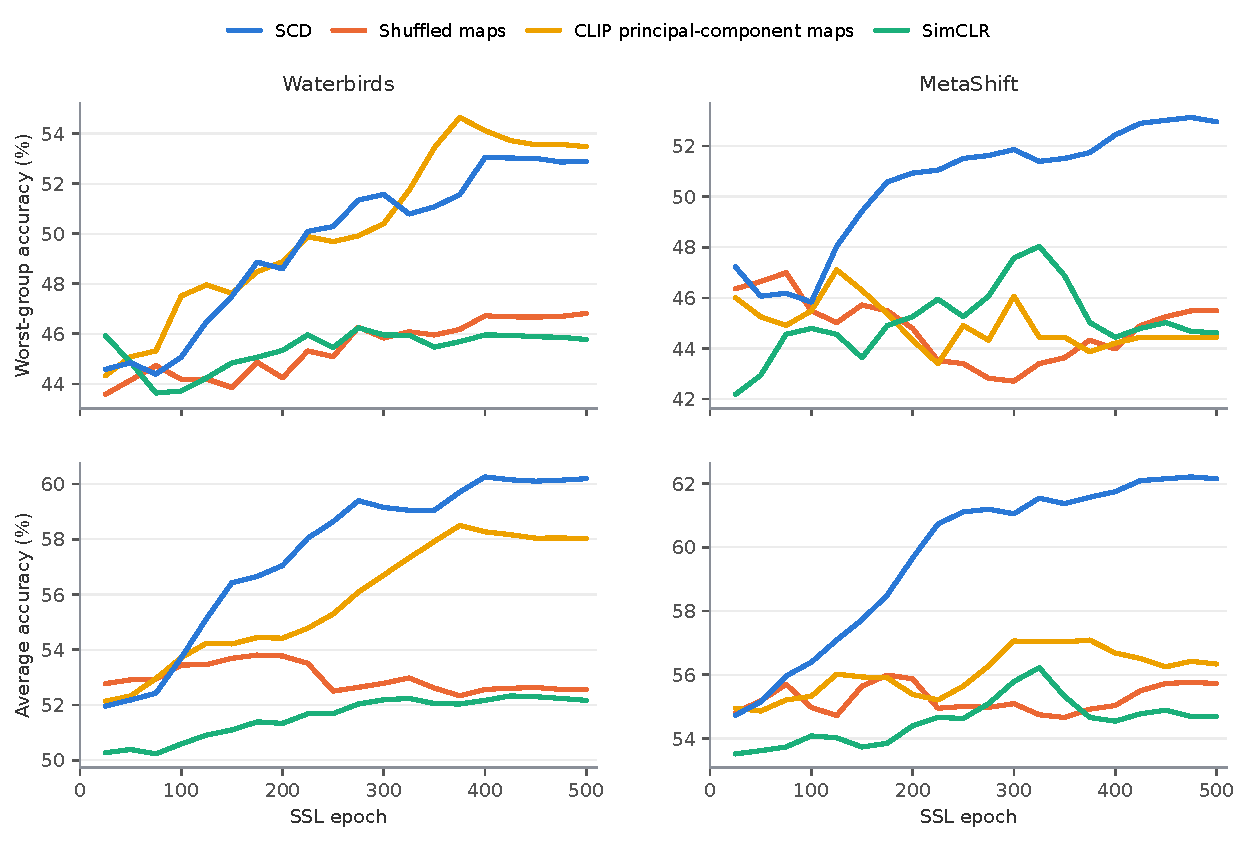
\includegraphics[width=\linewidth]{figures/spatial_training_curves.pdf}
\caption{Validation accuracy during SSL training for the methods of Table~\ref{tab:controls} except the image-level regression. Each line is the mean over seeds 1--4 of the periodic linear probes, run every 25 epochs, smoothed with a three-point moving average. Top: worst-group accuracy. Bottom: average accuracy. Table~\ref{tab:controls} reports the unsmoothed means of the last four probes.}
\label{fig:curves}
\end{figure}

\subsection{What do the concept maps capture?}
\label{sec:capture}
The MetaShift factors include scene concepts such as couch, lawn, beds, windows and bench next to the animal concepts; blankets, lawn, cats and fields win the most map cells (7.4\%, 6.6\%, 5.8\% and 5.6\%). On Waterbirds, bamboo, forest and tree stand win 37\% of the cells and the factor \emph{water bird} 6.2\%. Figure~\ref{fig:examples} shows the maps of four MetaShift training images and the $7\times7$ targets one SimCLR crop receives: the animal factors cover the animal and the scene factors its surroundings, whatever the group of the image.

\begin{figure}[htbp]
\centering
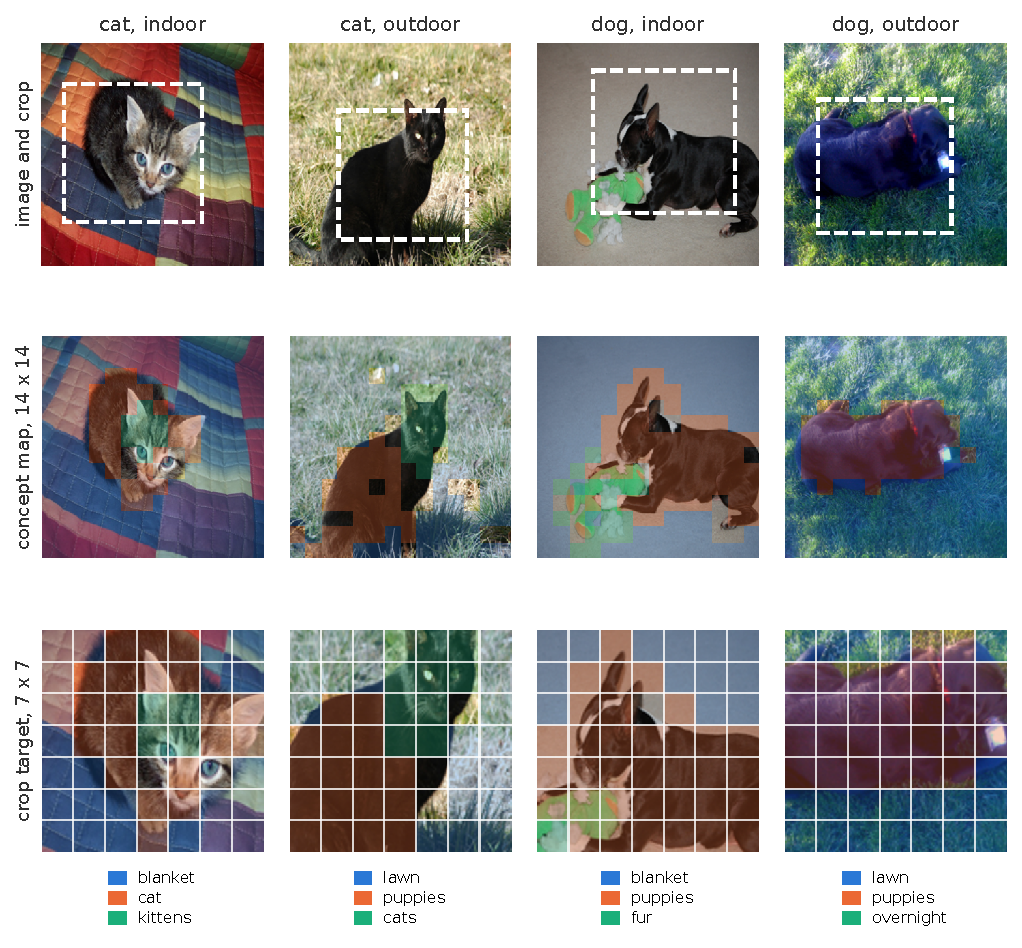
\includegraphics[width=\linewidth]{figures/spatial_map_examples.pdf}
\caption{Concept maps of MetaShift training images, one per group. Top: the image and one SimCLR crop (dashed). Middle: the factor that wins each cell of the $14\times14$ map, coloured for the image's three most frequent factors. Bottom: the crop's targets after warping to the student's $7\times7$ feature map. The images were chosen for illustration as the images of each group whose three leading factors cover most cells; class and group labels play no part in map construction or training.}
\label{fig:examples}
\end{figure}

The student carries the concepts to images outside the concept loss. On the held-out fifth of the training images, a ridge regression from the pooled student features explains 0.22 of the variance of the image-level factor responses on MetaShift and 0.26 on Waterbirds, against 0.13 and 0.17 with shuffled maps (Appendix~\ref{app:audit}). The scores on images in the concept loss agree with these (0.23 and 0.26), so the spatial loss generalizes where image-level distillation on MetaShift stored the targets of its training images. A concept ablation tests which concepts carry the MetaShift gain. It is an analysis with word lists we chose, outside the method. Over seeds 1--4, leaving out the 21 animal factors (cat, dog, breeds, pet, paws, fur) gives $46.61\pm5.75$ WGA and leaving out the 20 scene factors (couch, lawn, bed, window, desk, bench and others) $47.92\pm2.81$, against $53.04\pm5.75$ with all factors and $45.31\pm3.38$ with shuffled maps. Both ablations lose most of the gain and differ by less than the seed noise: the gain needs the full concept set.

Post-hoc labels show that the student strengthens the core feature without separating it from its usual context. The student's \emph{cat} factor scores 0.47 on unseen cats indoors and 0.07 on unseen cats outdoors, where CLIP features score 0.92 and 0.88. Each factor's residual on the other factors, the part a fused direction cannot predict, scores 0.00 in the student against 0.15 to 0.17 for CLIP. A location of the $7\times7$ map sees most of the view, so the cheapest predictor of ``cat here'' combines local evidence with the scene and the scene agrees with the cat on 88\% of the training images. SCD raises WGA because the balanced probe gains a usable core feature that SimCLR from scratch lacks and the spurious attribute stays as readable as before (Appendix~\ref{app:audit}).

\section{Limitations}
All results are validation results with the probe selected on the same split; held-out test runs with a locked probe are in progress. The study uses one concept vocabulary per dataset, one map construction and six (two on Spur-CIFAR10) student seeds; MetaShift's seed spread (5.4 WGA points) is as large as the gain over its controls on single seeds. The configuration with a 20\% hold-out became the main arm after it scored above the same loss with every image in it on validation (Waterbirds 49.53, MetaShift 46.70 WGA; Appendix~\ref{app:variants}); the difference lies within the seed spread and has no explanation yet. The group-balanced probe uses labels and group annotations, so only concept discovery, map construction and SSL are label-free.

Absolute accuracies are low, since ResNet-18 trains from scratch on 1,700 to 4,795 images: SCD reaches 60 to 61\% average accuracy on Waterbirds and MetaShift. LateTVG reports 55.4 and 59.3 WGA with SimCLR on Waterbirds and MetaShift under its own protocol \citep{hamidieh2024latetvg}; a first LateTVG run under our protocol reaches 47.9 on Waterbirds (one seed) and the matched multi-seed comparison is in progress. On Waterbirds, dense CLIP components match the concept maps, so the concept names add value only where the relevant contrast is a weak direction of CLIP.

The student keeps the training co-occurrence: its concept scores drop in the minority groups and the spurious attribute stays linearly readable (Waterbirds background probe 90.50\% WGA against 89.50\% for SimCLR). Variants that ask regions to keep their identity in foreign surroundings raise WGA further only when a text prompt types concepts as objects or scenes (Waterbirds 59.07 WGA with compositing), which the restriction of this work excludes; the prior-free variants we tried match or fall below SCD (Appendix~\ref{app:extensions}). The method depends on CLIP's external pretraining, its vocabulary coverage and its patch resolution: Spur-CIFAR10 images are upsampled from 32 to 448 pixels for the maps and CelebA, whose spurious attribute is gender, has no concept maps yet.

\begin{samepage}
\section{Conclusion}
SCD uses dense maps of SpLiCE concepts to supervise every location of a SimCLR student, through a regression cross-fitted between halves of the batch, with no labels and no concept type during pretraining. On Waterbirds, MetaShift and Spur-CIFAR10, its mean validation worst-group and average accuracies exceed those of SimCLR and of the same loss on shuffled maps. On MetaShift the named concepts beat dense CLIP components of the same width; on Waterbirds the two tie. The student's concepts still follow the training co-occurrence, so the results support a protocol-specific robustness gain from a stronger core feature, which locked test runs will confirm or revise.
\end{samepage}

\begingroup
\footnotesize
\setlength{\bibsep}{4pt plus 1pt}
\begin{thebibliography}{99}
\bibitem[Arefin et~al.(2024)]{arefin2024cobalt}
M.~R.~Arefin, Y.~Zhang, A.~Baratin, F.~Locatello, I.~Rish, D.~Liu and K.~Kawaguchi.
Unsupervised Concept Discovery Mitigates Spurious Correlations.
\emph{ICML}, pp.~1672--1688, 2024.
\url{https://proceedings.mlr.press/v235/arefin24a.html}.
\bibitem[Bertinetto et~al.(2019)]{bertinetto2019r2d2}
L.~Bertinetto, J.~F.~Henriques, P.~H.~S.~Torr and A.~Vedaldi.
Meta-learning with Differentiable Closed-Form Solvers. \emph{ICLR}, 2019.
\url{https://arxiv.org/abs/1805.08136}.
\bibitem[Bhalla et~al.(2024)]{bhalla2024splice}
U.~Bhalla, A.~Oesterling, S.~Srinivas, F.~P.~Calmon and H.~Lakkaraju.
Interpreting CLIP with Sparse Linear Concept Embeddings (SpLiCE).
\emph{NeurIPS}, 2024. \url{https://arxiv.org/abs/2402.10376}.
\bibitem[Chen et~al.(2020)]{chen2020simclr}
T.~Chen, S.~Kornblith, M.~Norouzi and G.~Hinton.
A Simple Framework for Contrastive Learning of Visual Representations.
\emph{ICML}, pp.~1597--1607, 2020.
\url{https://proceedings.mlr.press/v119/chen20j.html}.
\bibitem[Ghorbani et~al.(2019)]{ghorbani2019ace}
A.~Ghorbani, J.~Wexler, J.~Zou and B.~Kim.
Towards Automatic Concept-based Explanations. \emph{NeurIPS}, 2019.
\url{https://arxiv.org/abs/1902.03129}.
\bibitem[Hamidieh et~al.(2024)]{hamidieh2024latetvg}
K.~Hamidieh et~al.
Views Can Be Deceiving: Improved SSL Through Feature Space Augmentation.
\emph{ICLR}, 2024. \url{https://arxiv.org/abs/2406.18562}.
\bibitem[He et~al.(2016)]{he2016resnet}
K.~He, X.~Zhang, S.~Ren and J.~Sun.
Deep Residual Learning for Image Recognition. \emph{CVPR}, 2016.
\url{https://arxiv.org/abs/1512.03385}.
\bibitem[H\'enaff et~al.(2021)]{henaff2021detcon}
O.~J.~H\'enaff et~al.
Efficient Visual Pretraining with Contrastive Detection. \emph{ICCV}, 2021.
\url{https://arxiv.org/abs/2103.10957}.
\bibitem[Kim et~al.(2018)]{kim2018tcav}
B.~Kim, M.~Wattenberg, J.~Gilmer, C.~Cai, J.~Wexler, F.~Vi\'egas and R.~Sayres.
Interpretability Beyond Feature Attribution: Quantitative Testing with Concept Activation Vectors (TCAV).
\emph{ICML}, pp.~2668--2677, 2018. \url{https://proceedings.mlr.press/v80/kim18d.html}.
\bibitem[Kirichenko et~al.(2023)]{kirichenko2023dfr}
P.~Kirichenko, P.~Izmailov and A.~G.~Wilson.
Last Layer Re-Training is Sufficient for Robustness to Spurious Correlations.
\emph{ICLR}, 2023. \url{https://arxiv.org/abs/2204.02937}.
\bibitem[Koh et~al.(2020)]{koh2020cbm}
P.~W.~Koh, T.~Nguyen, Y.~S.~Tang, S.~Mussmann, E.~Pierson, B.~Kim and P.~Liang.
Concept Bottleneck Models. \emph{ICML}, pp.~5338--5348, 2020.
\url{https://proceedings.mlr.press/v119/koh20a.html}.
\bibitem[Krizhevsky(2009)]{krizhevsky2009cifar}
A.~Krizhevsky.
Learning Multiple Layers of Features from Tiny Images. Technical report, University of Toronto, 2009.
\bibitem[Lan et~al.(2024)]{lan2024clearclip}
M.~Lan et~al.
ClearCLIP: Decomposing CLIP Representations for Dense Vision-Language Inference.
\emph{ECCV}, 2024. \url{https://arxiv.org/abs/2407.12442}.
\bibitem[Lee et~al.(2019)]{lee2019metaoptnet}
K.~Lee, S.~Maji, A.~Ravichandran and S.~Soatto.
Meta-Learning with Differentiable Convex Optimization. \emph{CVPR}, 2019.
\url{https://arxiv.org/abs/1904.03758}.
\bibitem[Liang and Zou(2022)]{liang2022metashift}
W.~Liang and J.~Zou.
MetaShift: A Dataset of Datasets for Evaluating Contextual Distribution Shifts and Training Conflicts.
\emph{ICLR}, 2022. \url{https://arxiv.org/abs/2202.06523}.
\bibitem[Liu et~al.(2021)]{liu2021jtt}
E.~Z.~Liu, B.~Haghgoo, A.~S.~Chen, A.~Raghunathan, P.~W.~Koh,
S.~Sagawa, P.~Liang and C.~Finn.
Just Train Twice: Improving Group Robustness without Training Group Information.
\emph{ICML}, pp.~6781--6792, 2021.
\url{https://proceedings.mlr.press/v139/liu21f.html}.
\bibitem[Oikarinen et~al.(2023)]{oikarinen2023lfcbm}
T.~Oikarinen, S.~Das, L.~M.~Nguyen and T.-W.~Weng.
Label-Free Concept Bottleneck Models. \emph{ICLR}, 2023.
\url{https://arxiv.org/abs/2304.06129}.
\bibitem[Petryk et~al.(2022)]{petryk2022gals}
S.~Petryk et~al.
On Guiding Visual Attention with Language Specification. \emph{CVPR}, 2022.
\url{https://arxiv.org/abs/2202.08926}.
\bibitem[Radford et~al.(2021)]{radford2021clip}
A.~Radford et~al.
Learning Transferable Visual Models From Natural Language Supervision.
\emph{ICML}, pp.~8748--8763, 2021.
\url{https://proceedings.mlr.press/v139/radford21a.html}.
\bibitem[Ranzinger et~al.(2024)]{ranzinger2024radio}
M.~Ranzinger et~al.
AM-RADIO: Agglomerative Vision Foundation Model -- Reduce All Domains Into One.
\emph{CVPR}, 2024. \url{https://arxiv.org/abs/2312.06709}.
\bibitem[Robinson et~al.(2021)]{robinson2021shortcut}
J.~Robinson, L.~Sun, K.~Yu, K.~Batmanghelich, S.~Jegelka and S.~Sra.
Can contrastive learning avoid shortcut solutions? \emph{NeurIPS}, pp.~4974--4986, 2021.
\url{https://arxiv.org/abs/2106.11230}.
\bibitem[Ross et~al.(2017)]{ross2017rrr}
A.~S.~Ross, M.~C.~Hughes and F.~Doshi-Velez.
Right for the Right Reasons: Training Differentiable Models by Constraining their Explanations.
\emph{IJCAI}, 2017. \url{https://arxiv.org/abs/1703.03717}.
\bibitem[Ryali et~al.(2021)]{ryali2021background}
C.~K.~Ryali, D.~J.~Schwab and A.~S.~Morcos.
Characterizing and Improving the Robustness of Self-Supervised Learning through Background Augmentations.
\emph{arXiv:2103.12719}, 2021. \url{https://arxiv.org/abs/2103.12719}.
\bibitem[Sagawa et~al.(2020)]{sagawa2020groupdro}
S.~Sagawa, P.~W.~Koh, T.~B.~Hashimoto and P.~Liang.
Distributionally Robust Neural Networks for Group Shifts: On the Importance
of Regularization for Worst-Case Generalization.
\emph{ICLR}, 2020. \url{https://arxiv.org/abs/1911.08731}.
\bibitem[Shen et~al.(2022)]{shen2022unmix}
Z.~Shen et~al.
Un-Mix: Rethinking Image Mixtures for Unsupervised Visual Representation Learning.
\emph{AAAI}, 2022. \url{https://arxiv.org/abs/2003.05438}.
\bibitem[Tr\"auble et~al.(2021)]{trauble2021correlated}
F.~Tr\"auble et~al.
On Disentangled Representations Learned from Correlated Data.
\emph{ICML}, 2021. \url{https://arxiv.org/abs/2006.07886}.
\bibitem[von K\"ugelgen et~al.(2021)]{vonkugelgen2021content}
J.~von K\"ugelgen, Y.~Sharma, L.~Gresele, W.~Brendel, B.~Sch\"olkopf, M.~Besserve and F.~Locatello.
Self-Supervised Learning with Data Augmentations Provably Isolates Content from Style.
\emph{NeurIPS}, 2021. \url{https://arxiv.org/abs/2106.04619}.
\bibitem[Wang et~al.(2021)]{wang2021densecl}
X.~Wang et~al.
Dense Contrastive Learning for Self-Supervised Visual Pre-Training. \emph{CVPR}, 2021.
\url{https://arxiv.org/abs/2011.09157}.
\bibitem[Xiao et~al.(2021)]{xiao2021looc}
T.~Xiao, X.~Wang, A.~A.~Efros and T.~Darrell.
What Should Not Be Contrastive in Contrastive Learning. \emph{ICLR}, 2021.
\url{https://arxiv.org/abs/2008.05659}.
\bibitem[Xie et~al.(2021)]{xie2021pixpro}
Z.~Xie et~al.
Propagate Yourself: Exploring Pixel-Level Consistency for Unsupervised Visual Representation Learning.
\emph{CVPR}, 2021. \url{https://arxiv.org/abs/2011.10043}.
\bibitem[Yalavarthi et~al.(2026)]{yalavarthi2026dial}
B.~C.~Yalavarthi, N.~Ratha and V.~Govindaraju.
Label-Free Mitigation of Spurious Correlations in VLMs using Sparse Autoencoders.
\emph{ICLR}, 2026.
\href{https://proceedings.iclr.cc/paper_files/paper/2026/hash/359242d225d2fba218a85e147803f8b7-Abstract-Conference.html}{ICLR 2026 proceedings}.
\bibitem[Yang et~al.(2024)]{yang2024clipkd}
C.~Yang et~al.
CLIP-KD: An Empirical Study of CLIP Model Distillation. \emph{CVPR}, 2024.
\url{https://arxiv.org/abs/2307.12732}.
\bibitem[Yuksekgonul et~al.(2023)]{yuksekgonul2023pcb}
M.~Yuksekgonul, M.~Wang and J.~Zou.
Post-hoc Concept Bottleneck Models. \emph{ICLR}, 2023.
\url{https://arxiv.org/abs/2205.15480}.
\bibitem[Zhao et~al.(2021)]{zhao2021dilo}
N.~Zhao et~al.
Distilling Localization for Self-Supervised Representation Learning. \emph{AAAI}, 2021.
\url{https://arxiv.org/abs/2004.06638}.
\bibitem[Zhou et~al.(2022)]{zhou2022maskclip}
C.~Zhou, C.~C.~Loy and B.~Dai.
Extract Free Dense Labels from CLIP. \emph{ECCV}, 2022.
\url{https://arxiv.org/abs/2112.01071}.
\bibitem[Zhu et~al.(2023)]{zhu2023lassl}
W.~Zhu, S.~Liu, C.~Fernandez-Granda and N.~Razavian.
Making Self-supervised Learning Robust to Spurious Correlation via
Learning-speed Aware Sampling. \emph{arXiv:2311.16361}, 2023.
\url{https://arxiv.org/abs/2311.16361v2}.

\bibitem[Khosla et~al.(2020)]{khosla2020supcon}
P.~Khosla et~al.
Supervised Contrastive Learning. \emph{NeurIPS}, 2020.
\url{https://arxiv.org/abs/2004.11362}.


\end{thebibliography}
\endgroup

\clearpage
\appendix
\section{Concept and Training Configuration}
\label{app:provenance}
\begin{table}[ht]
\centering
\begin{tabularx}{\linewidth}{lX}
\toprule
Component & Setting \\
\midrule
CLIP teacher & OpenCLIP ViT-B/32, LAION-2B weights (\texttt{laion2b\_s34b\_b79k}) \\
SpLiCE & L1 penalty 0.25; LAION 10k vocabulary (MetaShift), Open Images v7 vocabulary (Waterbirds, Spur-CIFAR10) \\
Concept groups & Average linkage on raw text embeddings, text cosine 0.85; response correlation at least 0.5; concepts active on $[0.002,0.95]$ of images \\
Concept factors & Groups active on $[0.02,0.90]$ of images: 242 (Waterbirds), 130 (MetaShift), 147 (Spur-CIFAR10) \\
Concept maps & 448-pixel images, 224-pixel windows with stride 112; last block with query--query attention, without residual and feed-forward branch; softmax over factors at $T=0.01$; $14\times14$ grid \\
Targets & Standardized per factor over all images and cells; warped to each view by RoIAlign with its crop box and flip \\
Student features & ResNet-18 \texttt{layer4} map: $7\times7\times512$ (224-pixel views), $4\times4\times512$ (Spur-CIFAR10, 32-pixel views) \\
Cross-fit & Two halves of the batch's images, both views of an image in one half; unit-norm rows; absolute ridge $\rho=1$ \\
Loss weight & 0 up to epoch 10, linear warm-up to $\lambda_{\max}=5$ by epoch 20 \\
Hold-out & 20\% of training images with loss weight 0, the same images in every arm and seed \\
SSL & SimCLR, 500 epochs, batch 128, SGD with learning rate 0.01 decayed by 0.1 at epochs 350, 400 and 450, weight decay $10^{-4}$, temperature 0.05, float16 autocast, crop scale $[0.2,1]$ \\
Probe & Logistic regression with L2 coefficient 0.001 every 25 epochs; reported value is the mean of the last four probes \\
\bottomrule
\end{tabularx}
\end{table}

\section{Per-Seed and Per-Group Results}
\label{app:seedresults}
\begin{table}[htbp]
\centering\small
\setlength{\tabcolsep}{4pt}
\caption{Waterbirds validation, mean of the last four probes. Groups are in form $(y,a)$: landbird on land, landbird on water, waterbird on land and waterbird on water. Values are percentages.}
\begin{tabular}{lrrrrrrr}
\toprule
Method & Seed & Avg. & WGA & (0,0) & (0,1) & (1,0) & (1,1) \\
\midrule
SimCLR & 1 & 50.67 & 44.97 & 44.54 & 50.00 & 54.89 & 66.92 \\
SimCLR & 2 & 52.00 & 43.79 & 43.68 & 58.37 & 52.63 & 57.89 \\
SimCLR & 3 & 52.90 & 47.43 & 47.32 & 56.22 & 51.88 & 59.40 \\
SimCLR & 4 & 53.44 & 46.99 & 53.75 & 50.43 & 46.62 & 70.68 \\
SimCLR & 5 & 52.15 & 48.18 & 47.54 & 50.86 & 58.65 & 63.16 \\
SimCLR & 6 & 53.48 & 48.61 & 48.61 & 55.58 & 57.89 & 60.15 \\
\addlinespace
Shuffled maps & 1 & 56.46 & 50.19 & 53.32 & 60.52 & 50.38 & 57.89 \\
Shuffled maps & 2 & 53.29 & 47.54 & 47.75 & 56.87 & 59.40 & 54.14 \\
Shuffled maps & 3 & 52.61 & 44.91 & 45.61 & 59.44 & 51.88 & 55.64 \\
Shuffled maps & 4 & 48.02 & 44.27 & 43.90 & 45.28 & 55.64 & 60.15 \\
Shuffled maps & 5 & 53.19 & 48.07 & 48.18 & 56.22 & 54.14 & 58.65 \\
Shuffled maps & 6 & 53.17 & 50.00 & 50.75 & 56.22 & 51.13 & 54.14 \\
\addlinespace
SCD & 1 & 59.97 & 57.26 & 58.03 & 58.80 & 57.89 & 74.44 \\
SCD & 2 & 63.45 & 51.13 & 58.24 & 72.96 & 51.13 & 60.90 \\
SCD & 3 & 59.70 & 50.75 & 50.54 & 63.73 & 71.43 & 68.42 \\
SCD & 4 & 57.49 & 52.96 & 52.68 & 60.09 & 54.89 & 68.42 \\
SCD & 5 & 63.55 & 58.65 & 58.67 & 70.60 & 59.40 & 58.65 \\
SCD & 6 & 57.78 & 45.82 & 45.61 & 64.38 & 64.66 & 73.68 \\
\bottomrule
\end{tabular}
\end{table}

\begin{table}[htbp]
\centering\small
\setlength{\tabcolsep}{4pt}
\caption{MetaShift validation, mean of the last four probes. Groups are in form $(y,a)$: cat indoors, cat outdoors, dog indoors and dog outdoors. Values are percentages.}
\begin{tabular}{lrrrrrrr}
\toprule
Method & Seed & Avg. & WGA & (0,0) & (0,1) & (1,0) & (1,1) \\
\midrule
SimCLR & 1 & 56.34 & 50.69 & 59.72 & 50.00 & 58.33 & 55.56 \\
SimCLR & 2 & 55.30 & 44.79 & 50.00 & 62.50 & 44.44 & 63.89 \\
SimCLR & 3 & 48.09 & 31.60 & 48.61 & 30.56 & 50.00 & 61.11 \\
SimCLR & 4 & 59.46 & 52.08 & 61.11 & 51.39 & 58.33 & 66.67 \\
SimCLR & 5 & 53.82 & 44.44 & 62.50 & 45.83 & 44.44 & 63.89 \\
SimCLR & 6 & 57.99 & 42.36 & 58.33 & 41.67 & 61.11 & 70.83 \\
\addlinespace
Shuffled maps & 1 & 58.07 & 43.06 & 69.44 & 45.83 & 43.06 & 72.22 \\
Shuffled maps & 2 & 54.25 & 42.01 & 48.61 & 43.06 & 52.78 & 73.61 \\
Shuffled maps & 3 & 56.94 & 49.31 & 62.50 & 48.61 & 50.00 & 65.28 \\
Shuffled maps & 4 & 53.21 & 46.87 & 62.50 & 47.22 & 47.22 & 52.78 \\
Shuffled maps & 5 & 58.85 & 46.53 & 62.50 & 45.83 & 48.61 & 77.78 \\
Shuffled maps & 6 & 55.12 & 42.71 & 43.06 & 43.06 & 55.56 & 77.78 \\
\addlinespace
SCD & 1 & 66.06 & 60.42 & 69.44 & 61.11 & 68.06 & 66.67 \\
SCD & 2 & 58.85 & 50.69 & 59.72 & 51.39 & 51.39 & 75.00 \\
SCD & 3 & 61.63 & 54.17 & 62.50 & 52.78 & 58.33 & 70.83 \\
SCD & 4 & 62.33 & 46.87 & 69.44 & 47.22 & 55.56 & 79.17 \\
SCD & 5 & 60.33 & 48.61 & 63.89 & 48.61 & 56.94 & 73.61 \\
SCD & 6 & 57.73 & 45.83 & 58.33 & 45.83 & 52.78 & 72.22 \\
\bottomrule
\end{tabular}
\end{table}

\begin{table}[htbp]
\centering\small
\caption{Paired SCD differences in percentage points, mean of the last four probes.}
\begin{tabular}{rrrrrrrrr}
\toprule
& \multicolumn{4}{c}{Waterbirds} & \multicolumn{4}{c}{MetaShift} \\
& \multicolumn{2}{c}{vs. SimCLR} & \multicolumn{2}{c}{vs. shuffled maps} & \multicolumn{2}{c}{vs. SimCLR} & \multicolumn{2}{c}{vs. shuffled maps} \\
Seed & $\Delta$Avg. & $\Delta$WGA & $\Delta$Avg. & $\Delta$WGA & $\Delta$Avg. & $\Delta$WGA & $\Delta$Avg. & $\Delta$WGA \\
\midrule
1 & +9.30 & +12.29 & +3.50 & +7.07 & +9.72 & +9.72 & +7.99 & +17.36 \\
2 & +11.45 & +7.34 & +10.15 & +3.59 & +3.56 & +5.90 & +4.60 & +8.68 \\
3 & +6.80 & +3.32 & +7.09 & +5.84 & +13.54 & +22.57 & +4.69 & +4.86 \\
4 & +4.05 & +5.97 & +9.47 & +8.69 & +2.86 & $-$5.21 & +9.11 & +0.00 \\
5 & +11.41 & +10.47 & +10.36 & +10.57 & +6.51 & +4.17 & +1.48 & +2.08 \\
6 & +4.30 & $-$2.78 & +4.61 & $-$4.18 & $-$0.26 & +3.47 & +2.60 & +3.13 \\
\midrule
Mean & +7.88 & +6.10 & +7.53 & +5.26 & +5.99 & +6.77 & +5.08 & +6.02 \\
\bottomrule
\end{tabular}
\end{table}

On Spur-CIFAR10, SCD reaches $70.03/37.77$ and $68.61/38.49$ Avg./WGA on seeds 1 and 2, SimCLR $59.39/16.36$ and $59.71/14.89$ and the shuffled maps $56.41/15.84$ and $55.39/18.65$. Its 100 groups pair each class with each line colour.

\section{Map and Loss Details}\label{app:mapmath}

\paragraph{Map construction.}
Each 224-pixel window yields a $7\times7$ grid of ViT-B/32 patch embeddings. Window scores are spread onto a grid of 16-pixel cells, averaged where the nine windows of a 448-pixel image overlap and average-pooled to $14\times14$. The maps are stored in float16. The principal-component control projects the same dense patch embeddings, averaged over windows in the same way, onto their leading principal components, as many as the dataset has factors and standardizes them like the concept maps.

\paragraph{Warping and cross-fit.}
RoIAlign samples a $2\times2$ grid of points per output bin inside the view's crop box on the $14\times14$ map and returns a map of the feature-map size; a flipped view flips its targets. The halves of the cross-fit are the first and second half of the batch's images. Each half's regression solves one $C\times C$ system ($C=512$) over $64\cdot2\cdot hw$ rows, so the cost per step is that of a small matrix solve. The loss and the solve run in float32 outside the mixed-precision autocast. The run logs the held-out explained variance of the standardized targets, $1$ minus the mean held-out error. It starts near 0.4 at epoch 1, since maps are smooth and partly predictable from position and low-level statistics and ends at 0.44 to 0.48 for real maps against 0.39 to 0.41 for shuffled maps; only its rise above the shuffled control reflects concepts.

\paragraph{Implemented training objective.}
For normalized projection-head views $v_a$ in batch $B$, the implemented SimCLR term is
\begin{equation}
\mathcal{L}_{\mathrm{SimCLR}} = -\frac{\tau_C}{0.07} \frac{1}{2|B|}
\sum_a \log
\frac{
    \exp(v_a^\top v_{a^+}/\tau_C)
}{
    \sum_{b\neq a}\exp(v_a^\top v_b/\tau_C)
}.
\end{equation}
Here $a^+$ is the other view of the same image. The factor $\tau_C/0.07$ follows the SupCon implementation's temperature scaling \citep{khosla2020supcon}.

The spatial loss reads the \texttt{layer4} output through a forward hook, before global pooling and the projection head, so the probe sees the same backbone the loss shapes. Held-out images pass through the encoder with their batch and enter SimCLR; their weight of zero removes them from the fit and from the error. The weight $\lambda_{\max}=5$ comes from the grid 1, 3, 5 and 10 of the image-level regression on MetaShift and Waterbirds; weight 10 of the spatial loss adds nothing on two seeds (Appendix~\ref{app:variants}).

\section{Post-hoc Concept Audit}\label{app:audit}
After training, a ridge regression (ridge 10) maps the pooled features of the training images in the concept loss to each factor's image-level response, the cosine of the centred CLIP image embedding with the factor direction, standardized over images. The table reports the explained variance on the held-out fifth of the training images, averaged over factors and seeds. The residual score regresses each factor's part that the other factors leave unexplained. The group scores take the explained variance inside each $(y,a)$ group of the held-out images; labels enter only this evaluation. The held-out fifth holds 15 cats outdoors and 21 dogs indoors on MetaShift, so these group scores are coarse.

\begin{table}[htbp]
\centering\small
\setlength{\tabcolsep}{4pt}
\caption{Explained variance of the factor responses on the held-out training images, means over seeds 1--6 (principal-component maps: seeds 1--4). Group columns give the \emph{cat} factor on MetaShift (cat indoors, cat outdoors, dog indoors, dog outdoors) and the \emph{water bird} factor on Waterbirds (landbird on land, landbird on water, waterbird on land, waterbird on water).}
\begin{tabular}{llrrrrrr}
\toprule
Dataset & Features & All factors & Residuals & (0,0) & (0,1) & (1,0) & (1,1) \\
\midrule
MetaShift & SCD student & 0.22 & 0.00 & 0.47 & 0.07 & 0.10 & 0.47 \\
& Shuffled-map student & 0.13 & 0.00 & 0.24 & 0.08 & 0.19 & 0.29 \\
& Principal-component student & 0.16 & 0.00 & 0.32 & 0.05 & 0.17 & 0.34 \\
& CLIP & 0.74 & 0.15 & 0.92 & 0.88 & 0.83 & 0.91 \\
\addlinespace
Waterbirds & SCD student & 0.26 & 0.00 & 0.29 & 0.14 & $-$0.05 & 0.23 \\
& Shuffled-map student & 0.17 & 0.00 & 0.24 & $-$0.09 & $-$0.18 & 0.12 \\
& Principal-component student & 0.18 & 0.00 & 0.25 & $-$0.13 & $-$0.14 & 0.09 \\
& CLIP & 0.88 & 0.17 & 0.88 & 0.78 & 0.90 & 0.87 \\
\bottomrule
\end{tabular}
\label{tab:audit}
\end{table}

SCD raises the concept scores on unseen images by about 0.09 over the shuffled control on both datasets and reaches about 30\% of the CLIP score. The CLIP features score the \emph{cat} factor alike in all four groups; the student scores it where the factor and the scene agree (cats indoors and dogs outdoors, 0.47 each) and fails on cats outdoors (0.07). The \emph{water bird} factor drops in the same way on waterbirds on land. The residual scores stay at zero for every student: the student learns the part the factors share, which is the dataset's co-occurrence structure. A probe for the spurious attribute on the frozen features reaches $90.50\pm0.79$ WGA for SCD on Waterbirds against $89.50\pm1.05$ for SimCLR and $89.05\pm1.25$ for shuffled maps and $60.42\pm3.26$ on MetaShift against $56.48\pm6.37$ and $56.94\pm3.40$: SCD erases no background.

\begin{figure}[htbp]
\centering
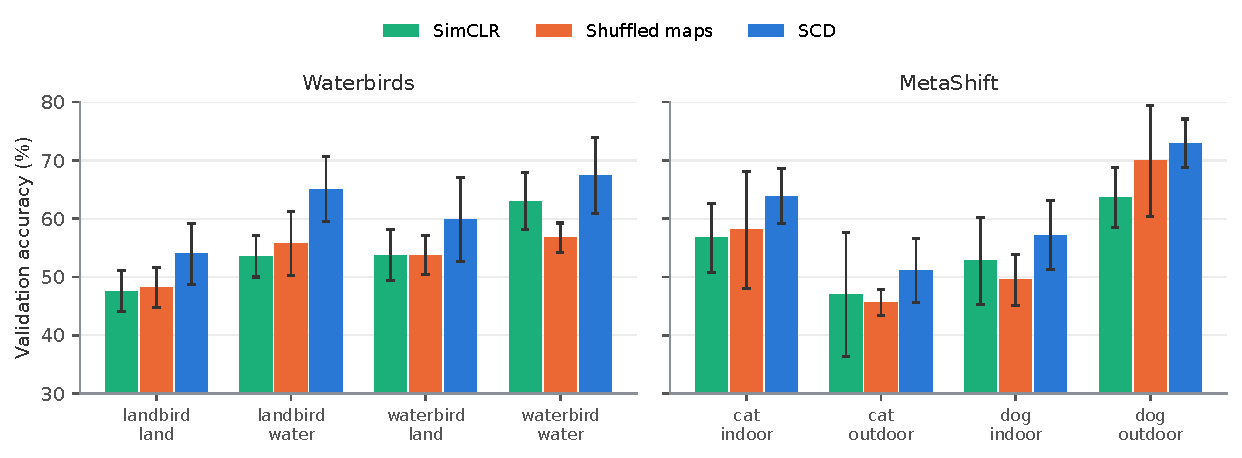
\includegraphics[width=\linewidth]{figures/spatial_group_accuracies.pdf}
\caption{Validation accuracy per (class, attribute) group, mean of the last four probes over seeds 1--6, with sample standard deviation across seeds. SCD raises every group on both datasets, the minority groups landbird on water and waterbird on land, cat outdoors and dog indoors included. Labels are used only for evaluation.}
\label{fig:groups}
\end{figure}

\section{Hold-out, Weight and Image-Level Variants}
\label{app:variants}
The image-level variants regress each image's factor values from the pooled backbone features with the same cross-fitted ridge, weight 5 and hold-out. They use the factors from a 5\% frequency band (70 on Waterbirds, 24 on MetaShift) and three kinds of target: standardized SpLiCE factor activations, the dense image-level responses of Appendix~\ref{app:audit} and as many principal components of the CLIP image embeddings.

\begin{table}[htbp]
\centering\small
\setlength{\tabcolsep}{4pt}
\caption{Validation Avg./WGA percentages, mean of the last four probes; seeds per dataset in brackets.}
\begin{tabular}{lll}
\toprule
Variant & Waterbirds & MetaShift \\
\midrule
SCD, 20\% hold-out, weight 5 & 60.32 / $52.76\pm4.68$ (1--6) & 61.15 / $51.10\pm5.44$ (1--6) \\
SCD without hold-out, weight 5 & 59.14 / $49.53\pm4.62$ (1--6) & 60.29 / $46.70\pm4.49$ (1--6) \\
SCD, 20\% hold-out, weight 10 & 61.84 / $53.53\pm4.92$ (1--2) & 60.55 / $48.26\pm5.89$ (1--2) \\
\addlinespace
Image-level SpLiCE factors & 57.96 / $50.37\pm8.98$ (1--4) & 61.68 / $47.22\pm3.93$ (1--2) \\
Image-level dense responses & 65.38 / $54.42\pm3.85$ (1--2) & 63.67 / $49.83\pm4.66$ (1--2) \\
Image-level CLIP components & 59.37 / $51.02\pm5.91$ (1--2) & 65.89 / $54.17\pm5.40$ (1--2) \\
\bottomrule
\end{tabular}
\label{tab:variants}
\end{table}

On Spur-CIFAR10 the image-level regression of 88 SpLiCE factors from the 2\% band at weight 1 reaches $68.66/29.39$ Avg./WGA with the hold-out and its shuffled control $58.16/22.29$ (seeds 1--2). The image-level variants rest on two seeds on MetaShift; their means lie within one seed spread of SCD and image-level CLIP components reach the highest MetaShift mean of the table. Image-level heads also store the targets of MetaShift's 1,700 training images: at weight 10 the score on images in the concept loss reaches 0.60 while the score on held-out images falls to 0.04. The spatial loss shows no such gap (0.23 against 0.22).

\section{Region, Mixing and Compositing Extensions}
\label{app:extensions}
We tested four extensions that ask concept regions of one image to keep their identity in other surroundings. Region contrast pools each view's feature map inside its two dominant concept regions and contrasts the regions of one concept across images, in the manner of DetCon \citep{henaff2021detcon}. Symmetric mixing keeps each concept region of a view with probability one half, fills the rest from another image and makes the mix a positive of both sources in proportion to their area \citep{shen2022unmix}. Per-group heads cluster the factors into 12 groups by the pixels they share, keep one group of a view on a donor's surroundings and train one projection head per group \citep{xiao2021looc}. Compositing pastes the object region of a view onto another image whose own objects are painted over \citep{zhao2021dilo,ryali2021background}; it decides which factors count as objects from their text similarity to object and scene prompts. All four run on top of SCD's spatial loss at weight 5 with the 20\% hold-out.

\begin{table}[htbp]
\centering\small
\caption{Validation Avg./WGA percentages, mean of the last four probes, seeds 1--4 (compositing on Waterbirds: seeds 1--6). The second column marks a step that types concepts as objects or scenes.}
\begin{tabular}{llll}
\toprule
Variant & Concept type & Waterbirds & MetaShift \\
\midrule
SCD (seeds 1--4) & no & 60.15 / $53.02\pm2.98$ & 62.22 / $53.04\pm5.75$ \\
Region contrast & no & 62.73 / $55.29\pm3.08$ & 64.28 / $50.00\pm6.48$ \\
\quad shuffled maps & no & 54.58 / $49.26\pm1.65$ & 54.25 / $42.45\pm6.74$ \\
Symmetric mixing & no & 56.02 / $49.18\pm2.46$ & 61.20 / $51.04\pm8.46$ \\
\quad rectangles instead of regions & no & 56.16 / $48.97\pm4.76$ & 61.44 / $51.82\pm3.41$ \\
Per-group heads & no & 59.36 / $52.38\pm2.87$ & 58.79 / $46.87\pm3.32$ \\
\quad one head for every pair & no & 55.06 / $42.87\pm4.81$ & 58.79 / $52.08\pm1.84$ \\
Compositing & yes & 64.73 / $59.07\pm7.09$ & 63.32 / $52.26\pm1.93$ \\
\quad another image's silhouette & yes & 62.47 / $54.22\pm6.13$ & 60.05 / $50.61\pm3.67$ \\
\quad context region kept & yes & 60.04 / $52.70\pm2.12$ & 60.13 / $49.31\pm1.94$ \\
\bottomrule
\end{tabular}
\label{tab:extensions}
\end{table}

Region contrast raises WGA on Waterbirds by 2.3 points, but its shuffled control gains as much over shuffled spatial maps and on MetaShift it loses 3.0 points. Symmetric mixing falls below SCD on both datasets and ties its rectangle control, so concept boundaries make no difference to it. Per-group heads beat their single-head control on Waterbirds and fall below it on MetaShift. Compositing gives the highest Waterbirds WGA of the study, ahead of SCD on all six seeds and keeping the context region in place of the object loses its gain. It reaches this through the object prior that the restriction of Section~3 excludes, so it serves as a reference for what a correct assumption about the spurious attribute adds.

\end{document}
